% figure1_chipflow_v5.tex — single-state with overlay layout.
% (a) pikv workflow (same as v1).
% (b) Single GPU row at top (FINAL state: 7 blue + 3 teal), single Host row at
%     bottom (with 3 teal chips marked as promoted/duplicated), RepairKV pill
%     vertically between them. Arrows: Host candidates -> score (in);
%     promote -> GPU (out). Signal s enters score from above-left.
%     Dashed link between the 3 teal chips in host and the 3 teal in GPU
%     (same entries, now in two places).
% Shared preamble for standalone Figure 1 variants.
\documentclass[border=8pt,tikz]{standalone}
\usepackage{amsmath}
\usepackage{amssymb}
\usepackage{tikz}
\usetikzlibrary{arrows.meta,positioning,calc,fit,shapes.geometric,backgrounds}
\usepackage{xcolor}
\usepackage[T1]{fontenc}
\usepackage{mathptmx}
\newcommand{\repairkv}{\textsc{RepairKV}}
\newcommand{\bbase}{\ensuremath{B_{\mathrm{base}}}}
\newcommand{\bmatch}{\ensuremath{B_{\mathrm{match}}}}

\begin{document}
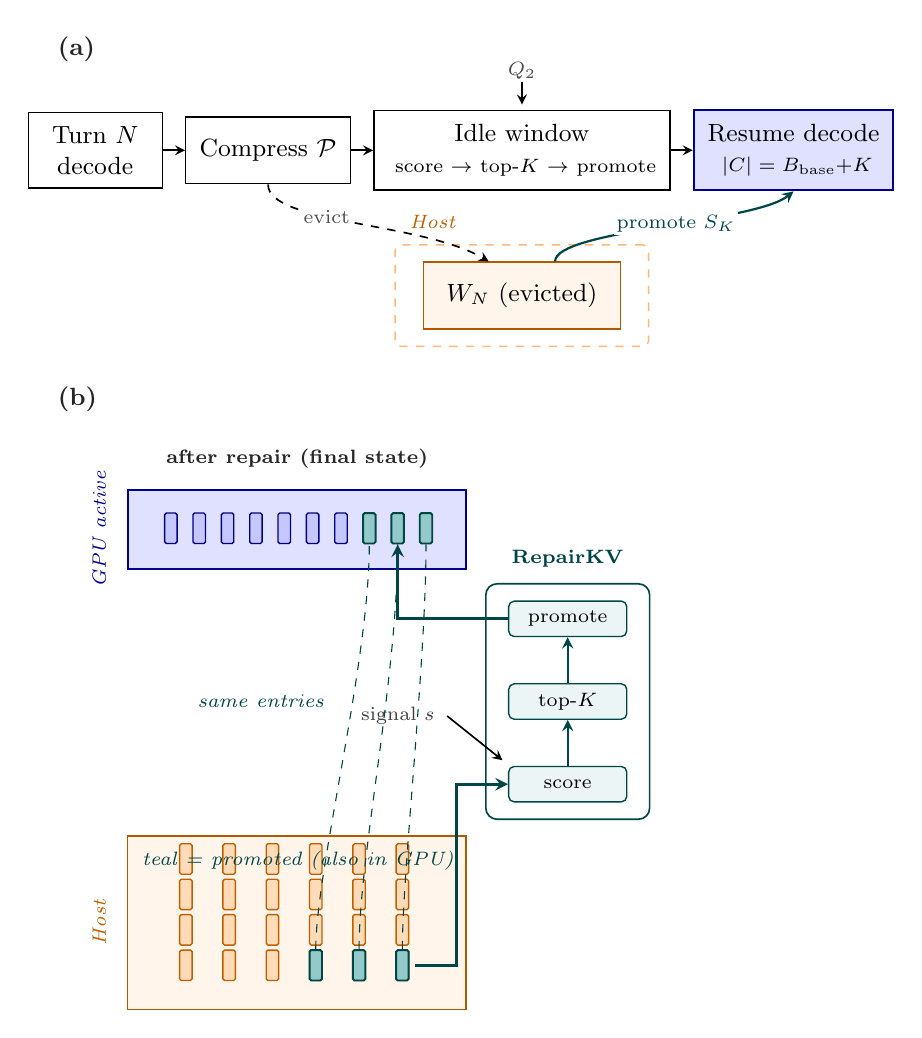
\begin{tikzpicture}[
  >=latex, line width=0.4pt,
  font=\small,
  box/.style={draw=black, fill=white, line width=0.5pt,
              inner sep=5pt, align=center, minimum height=0.85cm},
  active/.style={box, fill=blue!12, draw=blue!55!black, line width=0.7pt},
  store/.style={box, fill=orange!8, draw=orange!70!black},
  arr/.style={->, line width=0.6pt, draw=black, >=stealth},
  promarr/.style={->, line width=0.8pt, draw=teal!55!black, >=stealth},
  arrlabel/.style={font=\scriptsize, text=black!70, fill=white, inner sep=1pt},
  groupbox/.style={draw=orange!55, dashed, line width=0.5pt, rounded corners=2pt},
  grouplabel/.style={font=\scriptsize\itshape, text=orange!75!black},
  panellabel/.style={font=\bfseries\small, text=black!85},
  chip/.style={rounded corners=0.6pt, minimum width=4.5pt, minimum height=11pt,
               inner sep=0pt, line width=0.5pt},
  gpuchip/.style={chip, draw=blue!50!black, fill=blue!22},
  hostchip/.style={chip, draw=orange!75!black, fill=orange!28},
  promchip/.style={chip, draw=teal!55!black, fill=teal!42, line width=0.7pt},
  rkvmod/.style={draw=teal!55!black, fill=teal!8, line width=0.5pt,
                 rounded corners=2pt, inner sep=3pt, align=center,
                 font=\scriptsize, minimum width=1.5cm, minimum height=0.45cm},
  rowlabel/.style={font=\itshape\scriptsize},
  bigpromarr/.style={->, line width=1.0pt, draw=teal!55!black, >=stealth},
  overlaylink/.style={dashed, draw=teal!55!black, line width=0.4pt}
]
  % =================================================================
  % Panel (a) — pikv block diagram (same as v1)
  % =================================================================
  \node[panellabel, anchor=south west] at (0, 4.4) {(a)};

  \node[box, minimum width=1.7cm] (dN) at (0.6, 3.4) {Turn $N$\\decode};
  \node[box, minimum width=1.6cm, right=8pt of dN] (cmp) {Compress~$\mathcal{P}$};
  \node[box, minimum width=2.5cm, right=8pt of cmp] (idle)
       {Idle window\\{\scriptsize{} score~$\to$~top-$K$~$\to$~promote}};
  \node[active, minimum width=1.9cm, right=8pt of idle] (resume)
       {Resume decode\\{\scriptsize{} $|C|=\bbase{+}K$}};

  \draw[arr] (dN) -- (cmp);
  \draw[arr] (cmp) -- (idle);
  \draw[arr] (idle) -- (resume);

  \draw[arr] ([yshift=10pt]idle.north) -- ([yshift=2pt]idle.north);
  \node[arrlabel, anchor=south] at ([yshift=10pt]idle.north) {$Q_2$};

  \node[store, minimum width=2.5cm, below=0.9cm of idle] (wn) {$W_N$ (evicted)};
  \node[groupbox, fit=(wn), inner xsep=10pt, inner ysep=6pt] (hgroup) {};
  \node[grouplabel, anchor=south west]
       at ([xshift=2pt, yshift=2pt]hgroup.north west) {Host};

  \draw[arr, dashed]
       (cmp.south) .. controls ([yshift=-0.5cm]cmp.south)
                              and ([yshift=0.5cm]wn.north west) ..
       ([xshift=-12pt]wn.north)
       node[arrlabel, pos=0.4] {evict};

  \draw[promarr]
       ([xshift=12pt]wn.north) .. controls ([xshift=12pt, yshift=0.4cm]wn.north)
                                          and ([xshift=-0.5cm, yshift=-0.4cm]resume.south) ..
       (resume.south)
       node[arrlabel, text=teal!55!black, pos=0.55] {promote~$S_K$};

  % =================================================================
  % Panel (b) — single-state with overlay
  % Layout (centered):
  %   GPU row:  spans x = 1.0 .. 7.6, top-anchored
  %   Host row: spans x = 1.0 .. 7.6, bottom block
  %   RepairKV pill: centered between the two rows on the RIGHT side,
  %                  vertical (score bottom -> top-K -> promote top)
  %   Signal s: enters score from above-left
  % =================================================================
  \node[panellabel, anchor=south west] at (0, -0.05) {(b)};

  % --- GPU active row (TOP, final state) ---
  \node[active, minimum width=4.3cm, minimum height=1.0cm,
        anchor=north west] (gpu) at (1.0, -0.9) {};
  \node[rowlabel, text=blue!55!black, anchor=south, rotate=90]
       at ([xshift=-4pt]gpu.west) {GPU active};
  \node[font=\bfseries\scriptsize, text=black!85, anchor=south]
       at ([yshift=4pt]gpu.north) {after repair (final state)};

  % GPU chips: 7 blue + 3 teal (final state)
  \foreach \i in {1,...,7}{
    \pgfmathsetmacro{\xc}{0.36*\i + 0.20}
    \node[gpuchip] at ([xshift=\xc cm, yshift=-0.5cm]gpu.north west) {};
  }
  \foreach \i in {1,2,3}{
    \pgfmathsetmacro{\xs}{0.36*7 + 0.36*\i + 0.20}
    \node[promchip] (gpuTeal\i) at ([xshift=\xs cm, yshift=-0.5cm]gpu.north west) {};
  }

  % --- Host row (BOTTOM) ---
  \node[store, minimum width=4.3cm, minimum height=2.2cm,
        anchor=north west] (host) at (1.0, -5.3) {};
  \node[rowlabel, text=orange!75!black, anchor=south, rotate=90]
       at ([xshift=-4pt]host.west) {Host};

  % Host chips: 4 sub-rows of 6, with 3 teal candidates (promoted, also in GPU)
  \foreach \i in {1,...,6}{
    \foreach \r in {0,1,2,3}{
      \pgfmathsetmacro{\xh}{0.55*\i + 0.20}
      \pgfmathsetmacro{\yh}{-0.30 - 0.45*\r}
      \node[hostchip] at ([xshift=\xh cm, yshift=\yh cm]host.north west) {};
    }
  }
  % 3 teal candidates, clustered at bottom-right corner
  \pgfmathsetmacro{\xPa}{0.55*4 + 0.20} \pgfmathsetmacro{\yPa}{-0.30 - 0.45*3}
  \pgfmathsetmacro{\xPb}{0.55*5 + 0.20} \pgfmathsetmacro{\yPb}{-0.30 - 0.45*3}
  \pgfmathsetmacro{\xPc}{0.55*6 + 0.20} \pgfmathsetmacro{\yPc}{-0.30 - 0.45*3}
  \node[promchip] (hostTealA) at ([xshift=\xPa cm, yshift=\yPa cm]host.north west) {};
  \node[promchip] (hostTealB) at ([xshift=\xPb cm, yshift=\yPb cm]host.north west) {};
  \node[promchip] (hostTealC) at ([xshift=\xPc cm, yshift=\yPc cm]host.north west) {};

  % Note that the teal chips are shared
  \node[font=\scriptsize\itshape, text=teal!55!black, anchor=north west]
       at ([xshift=2pt, yshift=-2pt]host.north west)
       {\textcolor{teal!55!black}{teal} = promoted (also in GPU)};

  % --- RepairKV pill, vertical, BETWEEN the two rows (right side) ---
  % Vertical center: midpoint between GPU bottom (~ -1.9) and Host top (-5.3) = -3.6
  % Place pill on the RIGHT half so left side is clear for chip-link.
  \node[rkvmod, anchor=center] (mpromote) at (6.6, -2.55) {promote};
  \node[rkvmod, anchor=center] (mselect)  at (6.6, -3.6)  {top-$K$};
  \node[rkvmod, anchor=center] (mscore)   at (6.6, -4.65) {score};
  \draw[promarr] (mscore.north)  -- (mselect.south);
  \draw[promarr] (mselect.north) -- (mpromote.south);

  % RepairKV frame
  \node[draw=teal!55!black, line width=0.6pt, rounded corners=4pt,
        fit=(mpromote)(mscore), inner xsep=8pt, inner ysep=6pt] (rkvframe) {};
  \node[font=\scriptsize\bfseries, text=teal!55!black, anchor=south]
       at ([yshift=2pt]rkvframe.north) {\repairkv{}};

  % --- Signal s: enters score from above-left ---
  % A short angled arrow coming in from upper-left of the score module.
  \coordinate (sStart) at ([xshift=-22pt, yshift=18pt]mscore.north west);
  \draw[arr] (sStart) -- ([xshift=-2pt, yshift=2pt]mscore.north west);
  \node[font=\scriptsize, text=black!75, anchor=east]
       at ([xshift=-1pt]sStart) {signal $s$};

  % --- Flow arrows ---
  % Host teal cluster -> score (input). Up-and-right L-bend.
  \draw[bigpromarr]
       ([xshift=2pt]hostTealC.east)
       -- ([xshift=0.6cm]hostTealC.east)
       |- (mscore.west);

  % promote -> GPU teal cluster (output). Up-and-left L-bend to bottom of GPU teal.
  \draw[bigpromarr]
       (mpromote.west)
       -| ([xshift=0pt]gpuTeal2.south);

  % --- Dashed overlay links: 3 host teal <-> 3 GPU teal (same entries) ---
  % Use light dashed lines on the LEFT side of the figure so they don't
  % collide with the RepairKV pill on the right.
  \draw[overlaylink] (hostTealA.north) .. controls
       ([yshift=1.0cm]hostTealA.north) and ([yshift=-1.5cm]gpuTeal1.south) ..
       (gpuTeal1.south);
  \draw[overlaylink] (hostTealB.north) .. controls
       ([yshift=1.2cm]hostTealB.north) and ([yshift=-1.7cm]gpuTeal2.south) ..
       (gpuTeal2.south);
  \draw[overlaylink] (hostTealC.north) .. controls
       ([yshift=1.0cm]hostTealC.north) and ([yshift=-1.5cm]gpuTeal3.south) ..
       (gpuTeal3.south);

  % Tiny label on the overlay link (middle one)
  \node[font=\scriptsize\itshape, text=teal!55!black, fill=white, inner sep=1pt]
       at (2.7, -3.6) {same entries};

\end{tikzpicture}
\end{document}
